
\begin{figure}\flushleft
\begin{subfigure}[b]{0.4\textwidth}
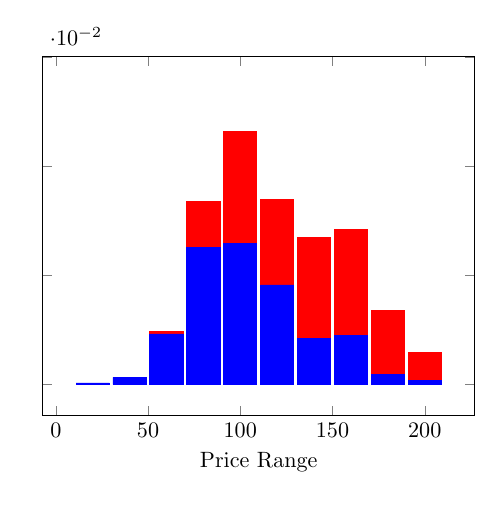
\begin{tikzpicture}[scale=0.8]
\begin{axis}[ybar stacked, bar width=15pt, ytick={}, yticklabels={}, xlabel={Price Range}, enlarge x limits=0.15, ymax=0.03]
\addplot+[ybar, fill=blue] plot coordinates {(20, 0.0001282051282051282) (40, 0.000641025641025641) (60, 0.004615384615384616) (80, 0.012564102564102566) (100, 0.012948717948717948) (120, 0.009102564102564102) (140, 0.004230769230769231) (160, 0.004487179487179487) (180, 0.0008974358974358973) (200, 0.0003846153846153846) };
\addplot+[ybar, fill=red] plot coordinates {(20, 0.0) (40, 0.0) (60, 0.0002564102564102564) (80, 0.004230769230769231) (100, 0.010256410256410256) (120, 0.00782051282051282) (140, 0.009230769230769232) (160, 0.009743589743589742) (180, 0.005897435897435897) (200, 0.002564102564102564) };
\end{axis}
\end{tikzpicture}
\caption{$n = 1$}
\end{subfigure}
\hspace{0.01\textwidth}
\begin{subfigure}[b]{0.4\textwidth}
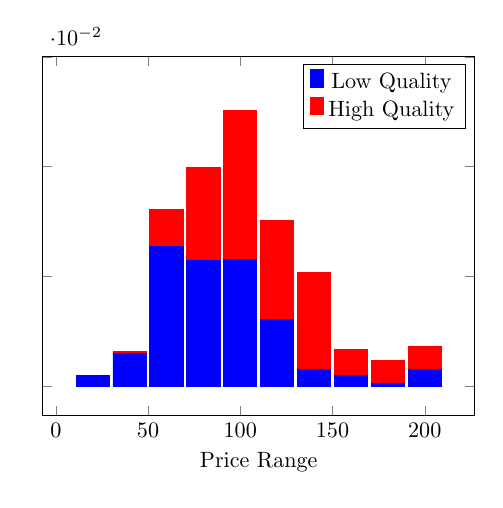
\begin{tikzpicture}[scale=0.8]
\begin{axis}[ybar stacked, bar width=15pt, ytick={}, yticklabels={}, xlabel={Price Range}, enlarge x limits=0.15, ymax=0.03]
\addplot+[ybar, fill=blue] plot coordinates {(20, 0.0009615384615384616) (40, 0.002980769230769231) (60, 0.012692307692307692) (80, 0.011442307692307693) (100, 0.011538461538461539) (120, 0.006057692307692307) (140, 0.0015384615384615385) (160, 0.0009615384615384616) (180, 0.00028846153846153843) (200, 0.0015384615384615385) };
\addplot+[ybar, fill=red] plot coordinates {(20, 0.0) (40, 0.0001923076923076923) (60, 0.0033653846153846156) (80, 0.008461538461538463) (100, 0.013557692307692307) (120, 0.009038461538461539) (140, 0.008846153846153846) (160, 0.002403846153846154) (180, 0.0020192307692307693) (200, 0.0021153846153846158) };
\legend{Low Quality, High Quality}
\end{axis}
\end{tikzpicture}
\caption{$n = 2$}
\end{subfigure}
\caption{Histogram of Low and High Quality Prices}
\label{pgrid_hist}
\end{figure}
